\documentclass{article}
\setlength{\parindent}{0ex}
\setlength{\parskip}{1em}
\usepackage[utf8]{inputenc} 
\usepackage{amsfonts}
\usepackage{amssymb}
\usepackage{amsmath}
\usepackage{amstext}
\usepackage{fancybox}
\usepackage{tikz}
\usepackage{tkz-euclide}
\usepackage{gensymb}
\usepackage{graphicx}
\usepackage{verbatim}
\usepackage{qtree}
\usepackage{scrextend}
\usepackage{multirow}
\usepackage{float}

\tikzset{main node/.style={circle,fill=blue!20,draw,minimum size=1cm,inner sep=0pt},
}

%Kodestyling \begin{lstlisting}
\usepackage{color}
\usepackage{listings}
\lstset{ %
language=C++,                % choose the language of the code
%basicstyle=\footnotesize,       % the size of the fonts that are used for the code
basicstyle=\ttfamily,
%numbers=left,                   % where to put the line-numbers
numberstyle=\footnotesize,      % the size of the fonts that are used for the line-numbers
stepnumber=1,                   % the step between two line-numbers. If it is 1 each line will be numbered
numbersep=5pt,                  % how far the line-numbers are from the code
backgroundcolor=\color{white},  % choose the background color. You must add \usepackage{color}
showspaces=false,               % show spaces adding particular underscores
showstringspaces=false,         % underline spaces within strings
showtabs=false,                 % show tabs within strings adding particular underscores
%frame=single,           % adds a frame around the code
tabsize=2,          % sets default tabsize to 2 spaces
captionpos=b,           % sets the caption-position to bottom
breaklines=true,        % sets automatic line breaking
breakatwhitespace=false,    % sets if automatic breaks should only happen at whitespace
escapeinside={\%*}{*)},          % if you want to add a comment within your code
mathescape
}

\usepackage{mathtools}
\DeclarePairedDelimiter\ceil{\lceil}{\rceil}
\DeclarePairedDelimiter\floor{\lfloor}{\rfloor}


\def\meta#1{\mbox{$\langle\hbox{#1}\rangle$}}
\def\macrowitharg#1#2{{\tt\string#1\bra\meta{#2}\ket}}

{\escapechar-1 \xdef\bra{\string\{}\xdef\ket{\string\}}}

\def\intro#1{{#1}{\cal I}}
\def\elim#1{{#1}{\cal E}}

\showboxbreadth 999
\showboxdepth 999
\tracingoutput 1


\let\imp\to
\def\elim#1{{{#1}{\cal E}}}
\def\intro#1{{{#1}{\cal I}}}
\def\lt{<}
\def\eqdef{=}
\def\eps{\mathrel{\epsilon}}
\def\biimplies{\leftrightarrow}
\def\flt#1{\mathrel{{#1}^\flat}}
\def\setof#1{{\left\{{#1}\right\}}}
\let\implies\to
\def\KK{{\mathsf K}}
\let\squashmuskip\relax

\graphicspath{ {images/} }
\usetikzlibrary{arrows}
\tikzset{
  leaf_/.style = {shape=rectangle,draw, align=center},
  node_/.style     = {shape=circle,draw,align=center}
}
\author{Rune Kok Nielsen (qkd362), Andreas Holm (jnh508)}
\title{Afløsningsopgave i fagområdet Modellering og Analyse af Data}
\DeclareMathOperator{\Ran}{Ran}
\DeclareMathOperator{\Dom}{Dom}
\begin{document}

\maketitle

\section{Klassificering}
Formålet med klassificering er at putte datapunkter bestående af et antal egenskaber i passende kategorier fra en prædifineret mængde af diskrete, beskrivende kategorier. Disse datapunkter er også kendt som tupler bestående af $(x,y)$, hvor $x$ er de givne egenskaber, og $y$ er punktets kategori. Klassificering består i definitionen af at finde en passende klassificeringsmodel, hvilket er en funktion $f$ der tager et datapunkt $x$ og returnerer den tilhørende kategori $y$.

Der findes adskillige teknikker til at bestemme en klassificeringsmodel. En sådan teknik beskriver en læringsalgoritme, der på basis af et træningssæt (et sæt af datapunkter med kendte kategorier) udleder en (evt. suboptimal) model.

Det er sjældent muligt at klassificere ethvert givent punkt korrekt ud fra de tilgængelige egenskaber, og vi har derfor brug for en måde at afgøre nøjagtigheden af den resulterende model. Denne nøjagtighed estimeres ved at klassificere et testsæt med modellen, og se på hvor stor en andel af datapunkterne der har fået den rigtige kategori. For at vise modellens nøjagtighed kan man beregne dens \textit{accuracy}, hvilket fortæller hvor præcis den er, eller man kan beregne dens \textit{error rate}, hvilke er det modsatte af \textit{accuracy} dvs. hvor mange forkerte punkter modellen har produceret.\\
For at beregne nøjagtigheden af en model, benytter vi et testsæt. Ligesom træningssættet er testsættet en mængde af datapunkter med kendte kategorier. Udregningerne består da i at klassificere punkterne i testsættet ved hjælp af modellen, og sammenligne punkternes kategorier som udregnet af modellen med deres egentlige kategorier, som vi kender i forvejen.\\
Det er essentielt at testsættet ikke overlapper med træningssættet, da dette vil tildele en for høj nøjagtighed til modellen. Har man f.eks.\ et meget lille træningssæt kan man nemt lave en model, som tilfældigvis passer perfekt på træningssættet, men som i realiteten er helt forkert. Tester man modellen på et testsæt som næsten overlapper fuldstændigt med træningssættet vil de overlappende punkter højst sandsynligt klassificeres korrekt, hvilket resulterer i meget høj nøjagtighed, selvom modellen i virkeligheden kun passer netop på træningssættet. 

For at udregne nøjagtiheden og fejlraten af klassificeringen bruger vi en \textit{confusion matrix}. En \textit{confusion matrix} ser formelt ud som i tabel 1 nedenfor. Her angiver $f_{ij}$ antallet af datapunkter i testsættet som tilhører klasse $i$, og blev klassificeret som klasse $j$. I det optimale tilfælde, hvor alle datapunkter klassificeres korrekt, har vi intuitivt $f_{ij}=0$ for $i\neq j$, hvilket manifesteres i en diagonal matrice.\\

\begin{table}[H]
\begin{center}
\begin{tabular}{cc|c|c|c|c|}
    & \multicolumn{5}{c}{Predicted Class} \\
    \cline{3-6}
     & & Class = 0 & Class = 1 & .. & Class = n \\
    \cline{2-6}
    \multicolumn{1}{c|}{\multirow{4}{*}{Actual Class}} & Class = 0 & $f_{00}$ & $f_{01}$ & .. & $f_{0n}$ \\
    \cline{2-6}
    \multicolumn{1}{c|}{} & Class = 1 & $f_{10}$ & $f_{11}$ & .. & $f_{1n}$ \\
    \cline{2-6}
    \multicolumn{1}{c|}{} & .. & .. & .. & .. & .. \\
    \cline{2-6}
    \multicolumn{1}{c|}{} & Class = n & $f_{n0}$ & $f_{n1}$ & .. & $f_{nn}$ \\
    \cline{2-6}
\end{tabular}
\caption{\textit{Confusion matrix}}
\end{center}
\end{table}

For at beregne vores \textit{accuracy} og \textit{error rate} kan vi finde antallet af korrekte- og forkerte forudsigelser ved at summere tallene på hhv. uden for diagonalen, og dividere værdierne med det totale antal klassificeringer. Vi får:\\

\begin{align*}
Accuracy &= \frac{Antallet \ af \ korrekte \ forudsigelser}{Det \ totale \ antal \ forudsigelser} \\
         &= \frac{\sum_{i=1}^{n}f_{ii}}{\sum_{i=1}^{n}\sum_{j=1}^{n}f_{ij}}
\end{align*}

\begin{align*}
Error \ rate &= \frac{Antallet \ af \ forkerte \ forudsigelser}{Det \ totale \ antal \ forudsigelser} \\
           &= \frac{\sum_{i=1}^{n}\sum_{j=1}^{n}e(i,j)}{\sum_{i=1}^{n}\sum_{j=1}^{n}f_{ij}}\\
           \text{hvor }e(i,j)&=
           \begin{cases} f_{ij} & \text{for } i\neq j \\
           0                                    & \text{ellers}      %
           \end{cases}
\end{align*}


Her gælder det klart at jo højere \textit{accuracy} desto bedre, og det modsatte gælder for \textit{error rate}. \\

\subsubsection{Problemer ved klassificering}
Det er ikke altid muligt at lave en perfekt klassificeringsmodel, som klassificerer ethvert givent punkt korrekt. F.eks. kunne datæn være utilstrækkelig til, at ramme alle tænkelige eksempler korrekt. Betragt træningssættet nedenfor. 

\begin{tabular}{c|c|c|c}
	Dyr & Lægger æg & Har et næb & Klasse\\
	\hline
	Pingvin & Ja & Ja & Fugl\\
	Aborre & Ja & Nej & Fisk\\
	Gorilla & Nej & Nej & Pattedyr\\
	Torsk & Ja & Nej & Fisk\\
	Due & Ja & Ja & Fugl\\
	Kat & Nej & Nej & Pattedyr
\end{tabular}

Datasættet indeholder kun to binære egenskaber, men ud fra træningssættet kan man nemt lave en model, som lader til at tildelte ethvert dyr i korrekt kategori (antaget at det ligger inde for en af de tre mulige klasser). Nedenfor ses et beslutningstræ, som klassificerer alle punkterne i træningssættet korrekt (mere om beslutingstræer i næste afsnit).

\begin{center}
	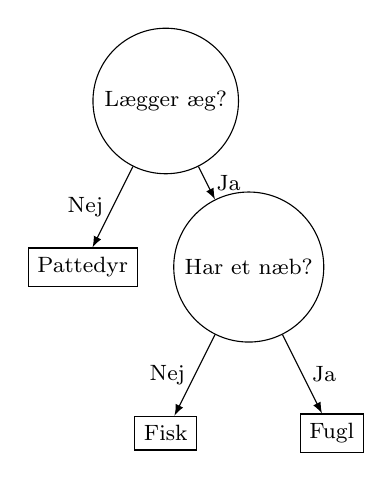
\begin{tikzpicture}
	[
	grow                    = down,
	sibling distance        = 6em,
	level distance          = 6em,
	edge from parent/.style = {draw, -latex},
	every node/.style       = {font=\footnotesize}
	]
	\node [node_] {Lægger æg?}
	child { node [leaf_] {Pattedyr}
		edge from parent node [left] {Nej} }
	child { node [node_] {Har et næb?}
		child { node [leaf_] {Fisk}
			edge from parent node [left]{Nej} }       
		child { node [leaf_] {Fugl}
			edge from parent node [right]{Ja} }
		edge from parent node [right] {Ja} };
	\end{tikzpicture}
\end{center}
Dette ser undertiden fint ud, men prøver man sætte et næbdyr ind i denne model, vil den blive klassificeret som en fugl (da den har et næb og lægger æg), selvom den egentlig er et pattedyr. Selvom vi egentlig har en model, som måske kan klassificere de fleste dyr korrekt, vil der være specielle tilfælde, hvor den skyder helt ved siden af. I dette eksempel kunne man muligvis løse problemet ved at indsamle flere egenskaber, og benytte et større træningssæt, men dette vil ikke altid være muligt, og der vil som sådan være situationer, hvor man ikke kan bygge en perfekt klassificeringsmodel.


\subsection{Beslutningstræer (Decision trees)}
Et eksempel på en klassificeringsteknik er gennem brug af beslutningstræer. Et beslutningstræ består af knuder og blade samt en rodknude. Et datapunkt kan da klassificeres ved at traversere træet startende i roden.

Hver knude består af et spørgsmål, som har en definitiv mængde svar, der kan besvares ud fra egenskaberne i et givent datapunkt. Ud fra svaret (altså datapunktets egenskaber) peger knuden videre til en ny knude eller et blad. Et blad repræsenterer den endelige kategori. I eksemplet i figur 1, kan der ses et eksempel på hvordan et beslutningstræ fungerer. I dette eksempel antager vi, at vi har fået en mængde, som indeholder enten biler, fly eller både. Vi starter med at spørge om det givet datapunkt har hjul, hvis nej må det være en båd, hvis ja kan det enten være en bil eller et fly, og derfor spørger vi igen, denne gang om det givet datapunkt har vinger, hvis ja er det et fly, og hvis nej må det være en bil. På denne måde har vi sikret os at vores datapunkt er kommet i den rigtige kategori.

\begin{figure}[H]
\begin{center}
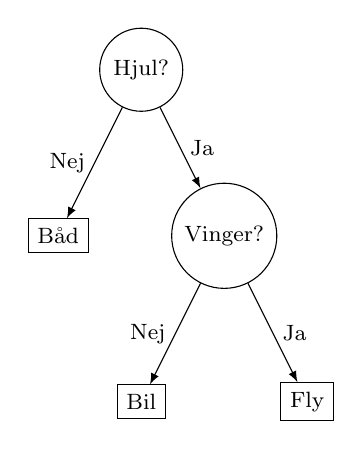
\begin{tikzpicture}
  [
    grow                    = down,
    sibling distance        = 6em,
    level distance          = 6em,
    edge from parent/.style = {draw, -latex},
    every node/.style       = {font=\footnotesize}
  ]
  \node [node_] {Hjul?}
    child { node [leaf_] {Båd}
      edge from parent node [left] {Nej} }
    child { node [node_] {Vinger?}
      child { node [leaf_] {Bil}
              edge from parent node [left]{Nej} }       
      child { node [leaf_] {Fly}
              edge from parent node [right]{Ja} }
              edge from parent node [right] {Ja} };
\end{tikzpicture}
\end{center}
\caption{Beslutningstræ}
\end{figure}

Et (muligvis suboptimalt) beslutningstræ kan konstrueres fra et træningssæt med Hunts algoritme. Algoritmen starter med en mængde af alle datapunkter i træningssættet. Hvis alle punkter i mængden har samme kategori, bliver denne mængde et blad i træet. Ellers stilles et spørgsmål om punkterne i mængden, og disse punkter samles i delmængder ud fra, hvordan de besvarer spørgsmålet. Spørgsmålet bliver en knude i træet, som peger på de nye delmængder, og algoritmen køres rekursivt på delmængderne. Effektiviteten og præcisionen af en sådan algoritme afhænger dermed af, at den kan stille de rigtige spørgsmål.


\subsubsection{Eksempel på modeludledning}
For at illustrere brugen af decision trees vil vi her vise et eksempel på, hvordan man ud fra et todimensionelt træningssæt og testsæt kan bygge og efterteste en klassificeringsmodel. Betragt træningssættet til venstre i figur 2 nedenfor. Tegner vi punkterne ind i et koordinatsystem opnår vi figuren til højre, hvor blå cirkler er A, røde plusser er B og gule stjerner er C.

\begin{figure}[H]
	\begin{minipage}[t]{0.27\linewidth}
		\begin{flushleft}
			\begin{tabular}{c|c|c}
				X & Y & Klasse\\
				\hline
				0.8 & 0.9 & A\\
				0.6 & 0.1 & B\\
				0.2 & 0.3 & C\\
				0.1 & 0.8 & C\\
				0.4 & 0.2 & B\\
				0.4 & 0.5 & A\\
				0.03 & 0.6 & C\\
				0.5 & 0. 3 & B\\
				0.6 & 0.7 & A\\
				0.45 & 0.8 & A\\
				0.8 & 0.7 & B\\
				0.28 & 0.3 & C\\
				0.1 & 0.05 & C
			\end{tabular}
		\end{flushleft}
	\end{minipage}
	\begin{minipage}[t]{0.25\linewidth}
		\begin{flushright}
			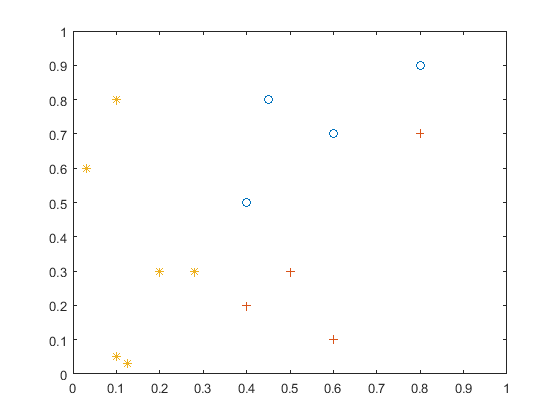
\includegraphics[width=9cm]{decision_tree_example_plot}
		\end{flushright}
	\end{minipage}
	\caption{\textit{Til venstre: eksempel på træningssæt. Til højre: plot af træningssættet.}}
\end{figure}
\begin{figure}[H]
	\begin{minipage}[t]{0.5\linewidth}
		\begin{flushleft}
			\ \\ \ \\
			Der er klare tendenser i, hvordan punkterne har fordelt sig. Ved at indtegne et par linjer kan vi tydeligt illustrere dette (figur 3).
		\end{flushleft}
	\end{minipage}
	\begin{minipage}[t]{0.25\linewidth}
		\begin{flushright}
			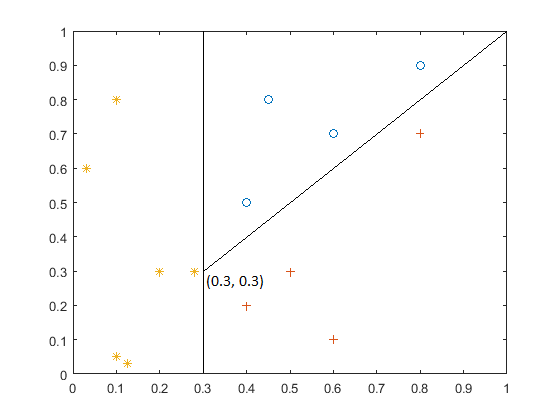
\includegraphics[width=8cm]{decision_tree_example_plot_splitted}
		\end{flushright}
	\end{minipage}
	\caption{\textit{Til højre: opdelt plot (se figur 2)}}
\end{figure}



Ud fra denne opdeling kunne det tyde på, at $f(x,y)=C$ for $x<0.3$, $f(x,y)=A$ for $0.3<x<y$ og $f(x,y)=B$ for $0.3<x$ og $y<x$. Med disse observationer kan vi bygge et beslutningstræ med Hunts algoritme.

Lad $D_t$ være hele træningssættet. Så indeholder $D_t$ punkter af alle klasser. Vi vælger nu en (\textit{attribute test condition}) at adskille punkterne på. For at få det mindste træ, starter vi med at teste om $x<0.3$, hvilket giver os en mængde $D_{t1}=\{p\ |\ class(p)=C\}$ for $0.3<x$ og $D_{t2}=\{p\ |\ class(p)\neq C\}$ for $x<0.3$. Da $D_{t1}$ kun indeholder en klasse bliver dette til et $C-$blad i træet, mens vi må teste rekursivt på $D_{t2}$.

Vi tester $D_{t2}$ for egenskaben $x<y$ og får en gruppe $D_{t3}=\{p\ | class(p)=A\}$ for $x<y$ og $D_{t4}=\{p\ |\ class(p)=B\}$ for $y<x$. Da begge disse grupper er rene (kun indeholder punkter af samme klasse) bliver disse til blade, og vi kan nu tegne vores beslutningstræ.

\begin{figure}[H]
	\begin{center}
		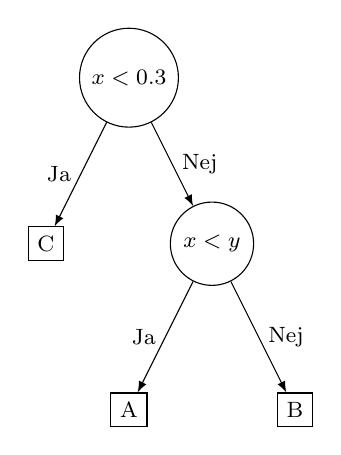
\begin{tikzpicture}
		[
		grow                    = down,
		sibling distance        = 6em,
		level distance          = 6em,
		edge from parent/.style = {draw, -latex},
		every node/.style       = {font=\footnotesize}
		]
		\node [node_] {$x<0.3$}
		child { node [leaf_] {C}
			edge from parent node [left] {Ja} }
		child { node [node_] {$x<y$}
			child { node [leaf_] {A}
				edge from parent node [left]{Ja} }       
			child { node [leaf_] {B}
				edge from parent node [right]{Nej} }
			edge from parent node [right] {Nej} };
		\end{tikzpicture}
	\end{center}
	\caption{\textit{Endeligt beslutningstræ}}
\end{figure}

Det er nu lykkedes at bygge en model, som kan opdele træningssættet korrekt. Dette er dog ingen garanti for, at modellen er korrekt. Modellen er bygget ud fra nogle antagelser, som holder gennem træningssættet, men det betyder ikke, at det holder i praksis. For at undersøge modellens nøjagtighed, vil vi bruge den til at klassificere et testsæt. I figur 5 har vi plottet et testsæt med opdelingen fra tidligere.

\begin{figure}[H]
	\begin{minipage}[t]{0.27\linewidth}
		\begin{flushleft}
			\begin{tabular}{c|c|c}
				X & Y & Klasse\\
				\hline
				0.2 & 0.01 & C\\
				0.28 & 0.1 & C\\
				0.1 & 0.2 & C\\
				0.4 & 0.5 & A\\
				0.5 & 0.8 & A\\
				0.9 & 0.95 & A\\
				0.5 & 0.4 & B\\
				0.8 & 0.2 & B\\
				0.6 & 0.5 & A\\
				0.7 & 0.1 & B\\
				0.5 & 0.12 & B\\
				0.12 & 0.75 & C
			\end{tabular} 
		\end{flushleft}
	\end{minipage}
	\begin{minipage}[t]{0.1\linewidth}
		\begin{flushright}
			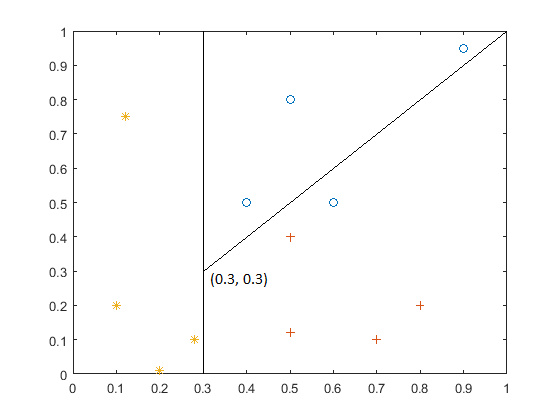
\includegraphics[width=9cm]{decision_tree_example_plot_test}
		\end{flushright}
	\end{minipage}
	\caption{\textit{Til venstre: Testsæt Til højre: Plot af testsæt}}
\end{figure}

Testsættet passer næsten overens, men der er et enkelt punkt som ikke overholder vores antagelse, så modellen er ikke perfekt. Helt konkret kan vi udregne en nøjagtighed baseret på vores resultat med testsættet. Ud af 12 punkter blev 11 punkter klassificeret korrekt, så vi regner os frem til en nøjagtihed $acc_M=\frac{11}{12}\approx0.92$


\section{Support Vector Machines (SVM)}

En SVM træningsalgoritme er en type klassifikationsteknik til binær klassifikation, som er specielt egnet til kontinuert data af mange dimensioner. Teknikken baseres på at finde et \textit{maximal margin hyperplane}, altså et hyperplan som deler datapunkterne op i to dele svarende til deres kategori, med maksimal margin til de nærmeste punkter. Dette hyperplan betegnes som modellens \textit{decision boundary}.

Formålet med at maksimere margin er at optimere modellens generaliseringsevne, og dermed opnå bedst mulig nøjagtighed, når nye punkter skal klassificeres. Hvis vores decision boundary har meget lille margin, er der intuitivt ikke plads til meget forskel på dataen sammenlignet med træningssættet. Dette koncept illustreres i eksemplet nedenfor.

Betragt træningssættet af todimensionelle punkter, markeret som plusser og cirkler afhængig af deres klasse (figur 6 til venstre). På figur 6 til højre er indtegnet to hyperplaner (sorte linjer) og deres margin (grå linjer), som begge deler træningssættet op uden fejl. Det er tydeligt at B2 har bredere margin end B1, og B2 er derfor objektivt den bedste løsning til problemet. Undersøger man selv dataen for en naturlig tendens i opdelingen, bliver det også tydeligt at se, at B2 følger denne tendens langt bedre end B1.

\begin{figure}[H]
	\begin{minipage}[t]{0.6\linewidth}
		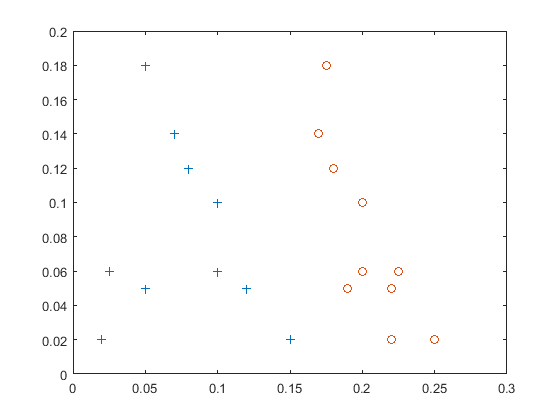
\includegraphics[width=7cm]{maximal_margin_hyperplane_1}
	\end{minipage}
	\begin{minipage}[t]{0.1\linewidth}
		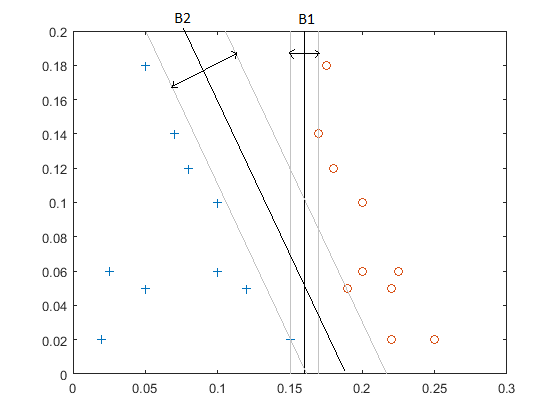
\includegraphics[width=7cm]{maximal_margin_hyperplane_2}
	\end{minipage}
	\caption{\textit{Til venstre: Træningssæt. Til højre: Opdeling af sættet med hyperplaner.}}
\end{figure}


\subsection{Linear SVM}
\subsubsection{Separable case}
I vores gennemgang af linear SVM vil vi kigge på et problem, hvor vi kan klassificere et dataset i to klasser. Vores inddeling kan beskrives mere formelt som $(x_i,y_i) \ i=1,2,...N$ hvor $x_i$ repræsenterer det i'te dataset. I disse eksempler vil $y_i \in \{-1,1\}$, dvs. at vi inddeler vores data i to klasser, enten $-1$ eller $1$.

For at finde punkter på vores grænse, kan vi opstille ligningen nedenfor, og de punkter, der opfylder ligningen, vil ligge på grænsen. De to variable $w$ og $b$ er parametre i modellen. For helt præcist at beskrive dem er $w$ en normal vektor til vores grænse \textit{decision boundary}, og $b$ er den vinkelrette afstand fra grænsen til origo.
$$w \cdot x + b = 0$$
På grafen nedenfor ses et eksempel på et plot af et dataset. Hvis der lå punkter på $B1$, ville de opfylde betingelserne for ligningen ovenfor.
\begin{center}
	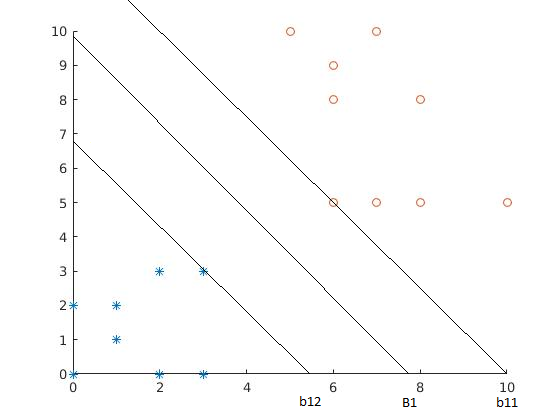
\includegraphics{svm_plot}
\end{center}

For punkter der ligger ved siden af grænsen kan vi opstille en gaffelfunktion, som kan ses nedenfor. De punkter der er mindre end $0$ ligger under grænsen, og vil blive klassificeret som $-1$, og de punkter der er større end $0$ ligger over grænsen, og vil blive klassificeret som $1$. Hvis vi kigger på grafen fra tidligere vil cirklerne blive kvalificeret som $1$, og stjernerne blive kvalificeret som $-1$.
$$
   y_i = \left\{
     \begin{array}{lr}
       1, & if \ w \cdot x_i + b > 0 \\
       -1, & if \ w \cdot x_i + b < 0
     \end{array}
   \right.
$$

Vi kan skalere vores $w$ og $b$ således at vi finder de punkter, der ligger på vores margener. Som det kan ses i den tidligere graf, vil det punkt som ligger på $b_{11}$ opfylde den første ligning, og det punkt, som ligger på b12 opfylde den anden ligning. 
$$b_{i1}: w \cdot x + b = 1$$
$$b_{i2}: w \cdot x + b = -1$$

Da vi gerne vil have de margener med den største afstand fra hinanden, kan vi omskrive de forudgående ligninger til at kunne beregne afstanden mellem margenerne. Dette kan vi gøre ved at indsætte de punkter, som ligger på den øvre og den nedre margen, og ved at trække de to ligninger fra hinanden, kan vi komme frem til den formel, som kan ses nedenfor. Her kan vi se, at afstanden mellem de to margener ($d$), kan findes ved $\frac{2}{||w||}$. Når vi senere hen skal til at optimere $d$, kan det let ses at for at finde den største afstand (altså maksimere $d$), skal vi minimere $w$. 
\begin{align*}
w \cdot (x_1 - x_2) = 2 \\
||w|| \times d = 2 \\
d = \frac{2}{||w||} \\
\end{align*}

For at træne vores SVM skal vi estimere $w$ og $b$ således at nedenstående betingelser er overholdt, de skal overholdes på den måde at de datapunkter som tilhører klassen $1$ skal overholde den første formel, og de dataset som tilhører klassen $-1$ skal overholde den anden formel. 
$$w \cdot x_i + b \geq 1 \ if \ y_i = 1$$
$$w \cdot x_i + b \leq -1 \ if \ y_i = -1$$

Formlerne ovenfor kan samles til formlen, som kan ses nedenfor, denne formel vil vi bruge i sammenhæng med optimering af $w$ og $b$. 
$$y_i(w \cdot x_i + b) \geq, \ i =1,2,...,N$$

For at opnå den største afstand mellem de to margener, kan vi opstille en objektiv funktion, som kan ses nedenfor. Da vi ønsker at maksimere $d$, er det klart, at den objektive funktion $f$ skal minimeres.  
$$f(w)=\frac{||w||^2}{2}$$

(To be completed)
Learning task:
$$\min\limits_{w} \frac{||w||^2}{2}$$
$$y_i(w \cdot x_i + b) \geq 1, i = 1,2,...,N$$

\subsubsection{Optimering}
For at optimere vores objektive funktion, skal vi bruge \textit{Lagrange multiplier}, \textit{Lagrange multiplier} er en metode der bruges til at finde en funktions minimum eller maksimum, og i dette tilfælde skal vi bruge den til at finde $f(w)=\frac{||w||^2}{2}$ minimum, da dette vil give os den bedste \textit{decision boundary}. Vi bruger \textit{Lagranges multiplier} da vores problem består af en kvadratisk objektiv funktion, og vores begrænsninger er lineære i parametrene $w$ og $b$, hvilket ender ud i at være et konvekst optimeringsproblem, og her bliver \textit{Langranges multiplier} brugt som standard.

For at kunne bruge \textit{Lagrange multipliers}, bliver vi nød til at omskrive vores objektive funktion, til en ny objektiv funktion, som tager højde for vores begrænsninger, den nye objektive funktion kendes også som en \textit{Lagrangian} funktion. Variablen $\lambda_i$ i den nye funktion er kendt som en \textit{Lagrange multiplier}. 
$$L_P = \frac{1}{2}||w||^2 - \sum\limits_{i=1}^N \lambda_i (y_i(w \cdot x_i + b) - 1)$$
Grunden til at vi har været nødsaget til at ændre vores objektive funktion fra $f(w) = \frac{||w||^2}{2}$ til den overstående objektive funktion er, at den tidligere funktion ville det let ses, at for at opnå den minimale værdi ville $w = 0$ være den bedste løsning, men denne løsning ville ikke holde da vores begrænsninger fra $y_i(w \cdot x_i + b) \geq 1, \ i =1,2,...,N$ ikke ville holde, og hvis vores uligheden ikke holder, vil vi ikke kunne finde en løsning til problemet. Det er her vores \textit{Lagrangian} funktion kommer i spil, da den inkorporerer vores betingelser i funktionen, og hvis betingelserne ikke holder, vil værdien af vores funktion stige, og dermed give et dårlige resultat.

For at kunne minimere vores \textit{Lagrangian} funktion, skal vi først lave to partielle differentieringer. Først differentierer vi i forhold til $w$, og derefter differentierer vi i forhold til $b$. Da vi ønsker at finde ekstremumspunkter, sættes de partielt differentierede til 0. Dette medfører resultatet nedenfor.
$$\frac{\partial L_p}{\partial w} = 0 \Rightarrow w = \sum\limits_{i=1}^N \lambda_i y_i x_i$$
$$\frac{\partial L_p}{\partial b} = 0 \Rightarrow \sum\limits_{i=1}^N \lambda_i y_i = 0$$
Selvom vi har fundet de partielt differentierede funktioner, er det stadig ikke muligt at finde $w$ og $b$, dette skyldes at vores definition af vores objektive funktion kun indeholder uligheder, og at \textit{Lagrange multiplier} skal bruge ligheder. Hvis vores definition havde indeholdt ligheder, ville det havde været muligt at finde værdierne til $w$, $b$ og $\lambda$ med de $N$ ligninger som vi har fundet. Men for at løse dette problem skal vi transformere vores uligheder til ligheder. Dette kan vi gøre med \textit{Karush-Kuhn-Tucker} betingelserne. Disse betingelser kan ses nedenfor.
$$\lambda_i \geq 0$$
$$\lambda_i[y_i(w \cdot x_i + b) - 1] = 0$$
Som det kan ses i vores nye ligheder, skal alle $\lambda_i$ være $0$ når $y_i(w \cdot x_i + b) \neq 0$, og ud fra dette ved vi at alle de punkter der ligger på $b_{i1}$ eller $b_{i2}$ har en \textit{Lagrange multiplier} $\lambda_i > 0$.  De punkter der ligger på $b_{i1}$ og $b_{i2}$ og opfylder betingelserne er også kendt som \textit{support vectors}.

Vores optimeringsproblem er stadig kompliceret grundet at vi har $w$, $b$ og $\lambda_i$. Vi kan simplificere problemet ved at bruge \textit{dual problem} metoden. Denne metode bruges ofte i sammenhæng med \textit{Lagrange mlutipliers}. Metoden transformerer vores \textit{Lagrangian} funktion til en funktion, som kun indeholder vores \textit{Lagrange multipliers}. Ved at indsætte konsekvenserne af de partielt differentierede sat til 0 i $L_P$ opnår vi vores \textit{dual problem} funktion som nedenfor.
$$L_D = \sum\limits_{i=1}^N \lambda_i - \frac{1}{2}\sum\limits_{i,j} \lambda_i \lambda_j y_i y_j x_j \cdot x_j$$
Der er to store forskelle på vores primære \textit{Lagrangian} funktion, og vores nye \textit{dual problem} funktion. Den første store forskel er at vores \textit{dual problem} kun indeholder vores trænings data samt vores \textit{Lagrange multipliers}, hvor vores primære \textit{Lagrangian} funktion også indeholder vores $w$ og $b$. Den anden store forskel er, at vores minimeringsproblem  er blevet til et maksimeringsproblem.
Løsningen af vores \textit{dual problem} kræver at vi finder værdierne af $\lambda_i$, hvilket opnås gennem $\textit{quadratic programming}$. Detaljerne ligger undertiden uden for emnet i denne rapport.\\
Efterat  vi har fundet $\lambda_i$ ved hjælp af \textit{quadratic programming} kan vi finde $w$ og $b$. Vi kan beskrive vores grænse med ligningen nedenfor.
$$( \sum\limits_{i=1}^N \lambda_i y_i x_i \cdot x) + b = 0$$

Når vi endelig er færdig med at beregne alle vores parametre for vores grænse, kan vi stille en funktionen op, som kan ses nedenunder, den funktion kan beregne hvilken klassifisering et givet datapunkt $z$ tilhører. Hvis $f(z) = 1$ vil $z$ blive klassificeret som $1$ ellers vil $z$ blive kvalificeret som $-1$. 
$$f(z) = sign(w \cdot z + b) = sign( \sum\limits_{i=1}^N \lambda_i y_i x_i \cdot z + b)$$

\subsubsection{Non-separable case}
I nogle tilfælde vil den bedste grænse (\textit{dicision boundary}) ikke altid klassificere alle punkter i vores dataset korrekt. Dette kan skyldes forskellige ting såsom fejl i træningsdata, eller at der er et enkelt dataset, som ikke holder sig til mønstret for dens klassificering. I disse tilfælde vil vi stadig prøve at opnå så stor en afstand mellem vores margener som muligt, selvom enkelte dataset bliver klassificeret forkert. Dette skyldes at hvis vi valgte en grænse, som ville opdele vores træningssæt uden fejl, ville grænsen ofte have en meget lille afstand mellems dens margener, og dette vil gøre at modellen ville være meget udsat for \textit{overfitting}. På grafen nedenfor ses et eksempel, hvor at $B2$ ville være den oplagte grænse at vælge, da den opdeler alt data korrekt, men vi også vælge $B1$ grundet at den har en større afstand mellem sine margener, og risikoen for \textit{overfitting} ville være mindre. 
\begin{center}
	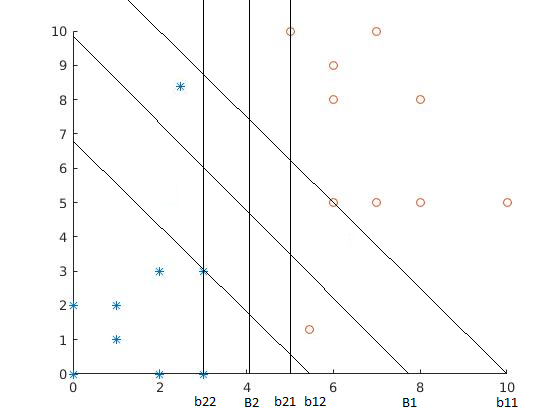
\includegraphics{svm_plot_1}
\end{center}
Grundet at vi har punkter der ikke er klassificeret rigtigt af vores grænse, vil vores tidligere ligninger ikke passe på alle vores dataset. For at rette dette introducerer vi \textit{slack variables} ($\xi$). Disse variabler skal placere de datapunkter der er kvalificeret forkert rigtigt, og dette gøres ved at addere eller substaktere (hvilke der skal bruges kommer an på hvor datapunktet er placeret) med vores nye variable ($\xi$). 

 Som det kan ses i vores to nye ligninger skal vi subtrakterer hvis vores dataset er placeret under grænsen, men den skal kvalificeres, som om den lå oven for grænsen, dette gør vi ved at subtrakterer højresiden af ligningen med vores \textit{slack variable}, med en værdi som gør at formlen er sand. Det samme gælder for det omvendte scenarie, men her bruges addition på højre siden af ligningen for at få ligningen til at blive sand.  
$$w * x_i + b \geq 1 - \xi_i \ if \ y_i = 1$$
$$w * x_i + b \leq 1 - \xi_i \ if \ y_i = -1$$
Bemærk $\forall i : \xi_i > 0$

For ikke bare at vælge en grænse med store margener, og så bare rette alle de forkerte klassificeret dataset til med \textit{slack variables}, introducerer vi en vægt for hvert datapunkt, som er kvalificeret forkert. Denne vægt kan ses i den modificerede objektive funktion nedenfor, bemærk at $C$ og $k$ bliver sat a brugeren (ofte vil $k = 1$ grundet simplicitet). Det ses klart at for hvert punkt, som er kvalificeret forkert, vil de valgte margener blive rangeret dårligere. 
$$f(w) = \frac{||w||^2}{2}+C(\sum\limits_{i=1}^N \xi_i)^k$$

\subsubsection{Optimering}
Optimering med vores \textit{slack variable} er næsten ens med vores optimering uden vores ekstra variable. Igen vil vi starte med at lave vores objektive funktion om til en \textit{Lagrangian} funktion.
$$L_P = \frac{1}{2}||w||^2 + C \sum\limits_{i=1}^N \xi_i - \sum\limits_{i=1}^N \lambda_i (y_i(w \cdot x_i + b) - 1 + \xi_i) - \sum\limits_{i=1}^N \mu_i \xi_i$$
For at forstå funktionen er det nemmest hvis man deler den op. Funktionen kan deles op i fire dele, hvor de to første dele er vores objektive funktion, som vi prøver at minimere, den tredje del  repræsenterer vores uligheder, er den sidste og fjerde del er kravet om at $\xi$ ikke må være negativt. 

Igen skal vi transformere vores uligheder til ligheder, og her vil vi igen bruge \textit{Karush-Kuhn-Tucker's} metode til at transformere dem. Nedenfor kan vores nye betingelser findes.
$$\xi_i \geq 0, \lambda_i \geq 0, \mu_i \geq 0$$
$$\lambda_i(y_i(w \cdot x_i + b) - 1 + \xi_i) = 0$$
$$\mu_i \xi_i = 0$$
Igen finder vi de partielt differentieret funktioner af $L_p$.
$$\frac{\partial L_p}{\partial w_j} = w_j - \sum\limits_{i=1}^N \lambda_i y_i x_{ij} = 0 \Rightarrow w_j = \sum\limits_{i=1}^N \lambda_i y_i x_{ij}$$
$$\frac{\partial L_p}{\partial b} = - \sum\limits_{i=1}^N \lambda_i y_i = 0 \Rightarrow \sum\limits_{i=1}^N \lambda_i y_i = 0$$
$$\frac{\partial L_p}{\partial \xi_i} = C - \lambda_i - \mu_i = 0 \Rightarrow \lambda_i + \mu_i = C$$
Hvis man som sidst indsætter vores nye ligninger ind i vores \textit{Lagrangian} funktion får vi igen et \textit{dual problem}, og dette er det samme som vi fandt frem til i det \textit{separable} tilfaelde. Den skiller sig lidt ud da vi har lidt flere betingelser, sidst havde vi bare at $\lambda_i \geq 0$, her har vi at $C \geq \lambda_i \geq 0$. Herfra er det den samme fremgangsmåde med \textit{quadratic programming} etc, som i det \textit{separable} tilfælde.
$$L_D = \sum\limits_{i=1}^N \lambda_i - \frac{1}{2}\sum\limits_{i,j}\lambda_i \lambda_j y_i y_j x_i \cdot x_j$$

\subsection{Ikke-lineær SVM}
Det er ikke altid muligt at definere en lineær opdeling af dataen. En naiv løsning på dette problem er, at transformere datapunkterne til et andet rum, hvor en lineær opdeling er mulig.

Antag at vi har en transformation $\Phi(x)$ fra det originale rum til et transformeret rum, hvor en lineær opdeling er mulig. Så kan vi genbruge vores viden fra det lineære tilfælde, og optimeringen er nogenlunde den samme. For at opnå den maksimale margin skal vi igen minimere funktionen 
$$f(w)=\frac{||w||^2}{2}$$
Under kravet at
$$y_i(w\cdot\Phi(x_i)+b)\geq 1,\text{ for }i=1,2..,N$$
Ligningen er næsten identisk med det lineære tilfælde, men vi optimerer nu med $\Phi(x_i)$ - altså $x_i$ i det transformerede rum.

Lagrange kan nu benyttes på samme måde som i det lineære tilfælde. Også her skal vi blot benytte de transfomerede punkter.

\begin{align*}
L_D&=\sum_{i=1}^{n}\lambda_i-\frac{1}{2}\sum_{i,j}\lambda_i\lambda_j y_iy_j\Phi(x_i)\cdot\Phi(x_j)
\end{align*}

Denne optimering kræver som man kan se udregningen af prikproduktet mellem samtlige par af punkter i det transformerede rum. Da dette kan være udregningsmæssigt tungt, og kræver at man kender en transformation der passer på det enkelte problem, vil man typisk bruge en anden tilgang kaldet \textit{kernel trick}, som tillader os at benytte kernefunktioner til at opnå et ækvivalent resultat.


\subsubsection{Kernefunktioner}
Lad $X=\{x_1..x_n\}\subset \chi_1$ være en mængde af $n$ vektorer i rummet $\chi_1$, og lad $\Phi:\chi_1\rightarrow\chi_2$. Da er en kernefunktion $k$ med feature mapping $\Phi$ en funktion der udregner det indre produkt af ethvert vektorpar $x_i,x_j\in X$ transformeret til $\chi_2$. Altså
\begin{equation}
k(x_i,x_j)=\langle\Phi(x_i),\Phi(x_j)\rangle
\end{equation}

Så definerer vi kernen $K$ som en $n\times n$-matrice med indre produkter af input vektorerne (en Gram matrice)
\begin{equation}
K=\left[\begin{array}{r r r}
\langle\Phi(x_1),\Phi(x_1)\rangle & ... & \langle\Phi(x_1),\Phi(x_n)\rangle\\
 & ... & \\
\langle\Phi(x_n),\Phi(x_1)\rangle & ... & \langle\Phi(x_n),\Phi(x_n)\rangle\\
\end{array}\right]\\
\end{equation}
Et indre produkt er per definition symmetrisk, så det følger at
\begin{equation}
K_{i,j}=\langle\Phi(x_i),\Phi(x_j)\rangle=\langle\Phi(x_j),\Phi(x_i)\rangle=K_{j,i}
\end{equation}
Hvilket viser at $K$ må være symmetrisk over diagonalen. 

Desuden vil en Gram matrice være positiv semidefinit. Dette kan bl.a. formaliseres under uligheden:
\begin{equation}
\forall c\in R^n,c^TKc\geq 0,\text{ for }c\neq 0
\end{equation}
Altså: for enhver vilkårlig ikke-nulvektor $c$ vil produktet af $c^TKc$ altså være ikke-negativt. Det følger at kernefunktionen $k$ er positiv semi-definit, hvilket er en central egenskab ved kernefunktioner.



Med denne definition kan $k$ nu erstatte prikproduktet og transformationerne i dual Lagrange problemet fra tidligere:
\begin{align*}
L_D&=\sum_{i=1}^{n}\lambda_i-\frac{1}{2}\sum_{i,j}\lambda_i\lambda_j y_iy_jK(x_i,x_j)
\end{align*}


\end{document}